% Section 4: a chat log starts at the first prompt. Work done before it is
% outside the log, and has to come from the written work and interviews.
\documentclass[tikz,border=6pt]{standalone}
% Shared art for "Asking a chatbot to confirm a proof": the palette and the
% chatbot, worksheet and chat bubble of the SPLICE talk's summary figure and
% the Builder tile, so the post, the talk page and the lab page look alike.
\usetikzlibrary{arrows.meta,decorations.pathmorphing,calc}
\definecolor{ink}{HTML}{1B2430}
\definecolor{rule}{HTML}{9AA4AB}
\definecolor{edge}{HTML}{5A646E}
\definecolor{tint}{HTML}{F7E9E9}
\definecolor{red}{HTML}{8B2E2E}
\tikzset{
  flow/.style={-{Stealth[length=3.4mm]}, draw=edge, line width=1.3pt},
  lbl/.style={font=\sffamily\Large, text=ink, align=center},
  note/.style={font=\sffamily\large, text=edge, align=center},
  title/.style={font=\sffamily\bfseries\LARGE, text=ink},
  chip/.style={font=\sffamily\bfseries\large, text=white, fill=red,
               rounded corners=3pt, inner sep=5pt},
}
% A worksheet: lower-left (#1,#2), width #3, height #4. #5 is the colour of the
% third line: red for a perturbed question, rule for plain work.
\newcommand{\sheet}[5]{%
  \fill[white, draw=edge, line width=1.2pt, line join=round]
    (#1,#2) -- ++(#3,0) -- ++(0,#4-0.4) -- ++(-0.4,0.4) -- ++(-#3+0.4,0) -- cycle;
  \draw[edge, line width=1.2pt, line join=round] (#1+#3-0.4,#2+#4) -- ++(0,-0.4) -- ++(0.4,0);
  \foreach \f in {0.76,0.58,0.24}
    \draw[rule, line width=1.5pt, line cap=round] (#1+0.28,#2+\f*#4) -- ++(#3-0.56,0);
  \draw[#5, line width=1.7pt, line cap=round, decorate,
        decoration={zigzag, segment length=2.2mm, amplitude=0.7mm}]
    (#1+0.28,#2+0.41*#4) -- ++(#3-0.56,0);}
% The chatbot's head, centred on (#1,#2).
\newcommand{\chatbot}[2]{%
  \fill[red] (#1-0.8,#2-0.62) rectangle ++(1.6,1.24);
  \fill[white] (#1-0.4,#2+0.12) circle (0.16);
  \fill[white] (#1+0.4,#2+0.12) circle (0.16);
  \draw[white, line width=1.3pt] (#1-0.3,#2-0.3) -- ++(0.6,0);
  \draw[red, line width=1.5pt] (#1,#2+0.62) -- ++(0,0.4);
  \fill[red] (#1,#2+1.1) circle (0.13);}
% A student: head and shoulders, centred on (#1,#2).
\newcommand{\student}[2]{%
  \fill[edge] (#1,#2+0.45) circle (0.42);
  \fill[edge] (#1-0.8,#2-0.75) .. controls (#1-0.8,#2+0.1) and (#1+0.8,#2+0.1) .. (#1+0.8,#2-0.75) -- cycle;}
% A rubric card, failed, lower-left (#1,#2), side #3.
\newcommand{\failcard}[3]{%
  \fill[white, draw=edge, line width=1.2pt, rounded corners=3pt] (#1,#2) rectangle ++(#3,#3);
  \draw[red, line width=2.6pt, line cap=round]
    (#1+0.25*#3,#2+0.25*#3) -- ++(0.5*#3,0.5*#3) (#1+0.25*#3,#2+0.75*#3) -- ++(0.5*#3,-0.5*#3);}

\begin{document}
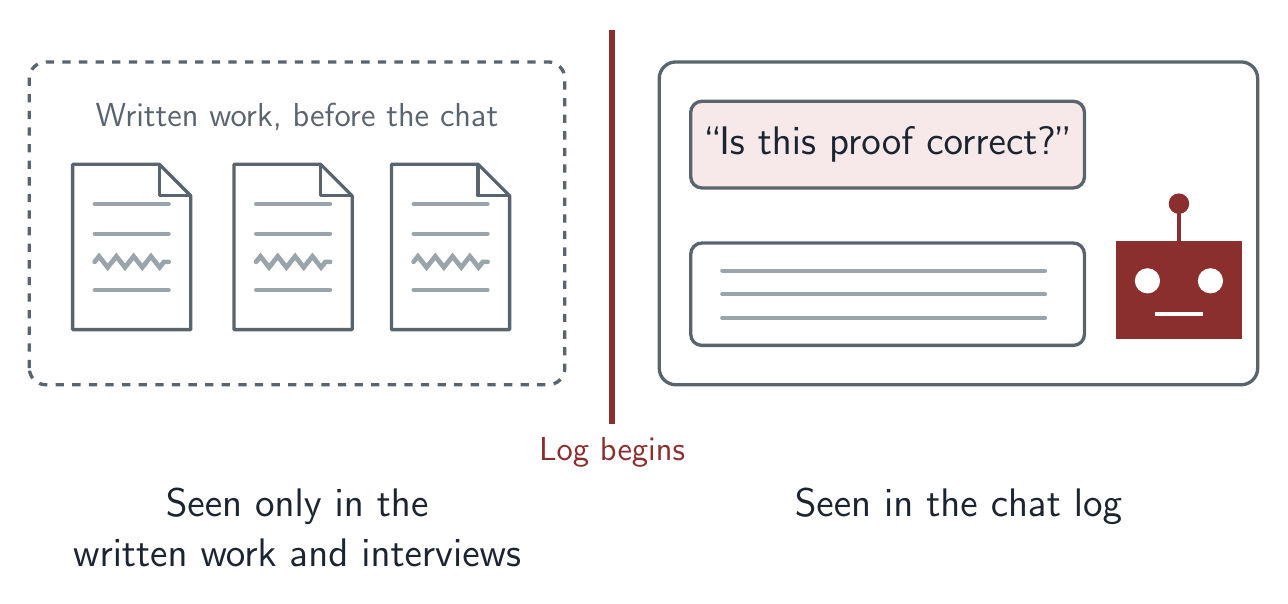
\begin{tikzpicture}[font=\sffamily]
  % before the prompt: written work, outside the log
  \draw[edge, line width=1.2pt, dashed, rounded corners=6pt] (0,0.9) rectangle (6.8,5.0);
  \sheet{0.55}{1.6}{1.5}{2.1}{rule}
  \sheet{2.6}{1.6}{1.5}{2.1}{rule}
  \sheet{4.6}{1.6}{1.5}{2.1}{rule}
  \node[note, anchor=south] at (3.4,4.0) {Written work, before the chat};
  % the moment the log begins
  \draw[red, line width=2pt] (7.4,0.4) -- (7.4,5.4);
  \node[note, anchor=north, text=red] at (7.4,0.35) {Log begins};
  % the log
  \fill[white, draw=edge, line width=1.2pt, rounded corners=6pt] (8.0,0.9) rectangle (15.6,5.0);
  \fill[tint, draw=edge, line width=1.2pt, rounded corners=4pt] (8.4,3.4) rectangle (13.4,4.5);
  \node[lbl] at (10.9,3.95) {``Is this proof correct?''};
  \chatbot{14.6}{2.1}
  \fill[white, draw=edge, line width=1.2pt, rounded corners=4pt] (8.4,1.4) rectangle (13.4,2.7);
  \foreach \y in {2.35,2.05,1.75} \draw[rule, line width=1.5pt, line cap=round] (8.8,\y) -- (12.9,\y);
  % what each side can show
  \node[lbl, anchor=north] at (3.4,-0.3) {Seen only in the\\written work and interviews};
  \node[lbl, anchor=north] at (11.8,-0.3) {Seen in the chat log};
\end{tikzpicture}
\end{document}
